\chapter{Hello Adventure World} 

\section{Introduction}

A program is basically a set of instructions what to do. There are different programming languages we can write such instructions in -- Python is one of them. Other languages are for example Java, C, C++, Swift -- by now (October 2018) probably close to 300 different programming languages exist! But, we will just focus on Python for the moment. 

Python is actually more than "just" a language. It is also a program that can interpret your program and then translate it into instructions for your computer to execute. Let us see that in action right away. 

Open a terminal, type in \textbf{\texttt{idle3 \&}} after the \$-prompt, and press return: 

\begin{itemize}
\item[\$] \textbf{\texttt{idle3 \&}}
\end{itemize}

Up pops a little window, like the one below.  
 
\begin{figure}[h]
\centerline{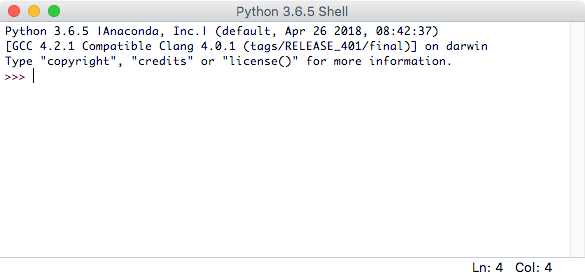
\includegraphics[scale=.70]{images/p1ch1-idle3.png}}
\caption{The Python IDLE3 interactive editor}
\end{figure}

This is the \texttt{idle3} window. It is an interactive editor for Python. Everything you type in is immediately interpreted and executed -- so you can see right away what it does! 
Let's see this at work. After the "$>>>$" prompt in the editor, type in the following: 

\begin{itemize}
\item[$>>>$] \textbf{\texttt{print("Hello Adventure World!")}}
\end{itemize}

And there you go! Right below your command, \texttt{idle3} shows the text "Hello Adventure World!" -- you have written \emph{and} executed (or "ran") your first line of Python code!

\begin{itemize}
\item[$>>>$] \texttt{print("Hello Adventure World!")}\\
	\textbf{\texttt{Hello Adventure World!}}
\end{itemize}

Feel free to try out more -- how do you imagine your adventure would start? Where does the player start, what does he -- or she -- see, smell, feel? 

\begin{itemize}
\item[$>>>$] \textbf{\texttt{print("You are in a dark, spooky house, hidden deep in the forest. \\ 
		   There is only one door to the outside, and it is locked. You hear \\ 
		   strange, creaky sounds. What do you do?")}}
\end{itemize}
   
Sometimes such a long piece of text looks kind of awkward. If you want to break things up a little, you can insert a \texttt{$\backslash$n} or "new line" in your text. For example, if we want to have each sentence start at a new line, we can achieve that as follows: 

\begin{itemize}
\item[$>>>$] \textbf{\texttt{print("You are in a dark, spooky house, hidden deep in the forest.$\backslash$n\\ 
		   There is only one door to the outside, and it is locked.$\backslash$n \\
		   You hear strange, creaky sounds.$\backslash$n\\
		   What do you do?$\backslash$n")}}
\end{itemize}
   

\section{Your First Real Program}    
   
The \texttt{idle} interactive editor is useful to try a couple of things out, and see what they do. However, you can only do things line by line, and have to retype everything if you want to try again! In this section move to using \textit{Atom}, a so-called "interactive development environment" or IDE. We will use editor to type in programs, run them, and store versions in \texttt{git}.

Start up \textit{Atom}, and click on the "Welcome Guide" tab. The window will look something like what you see below. 

\begin{figure}[h]
\centerline{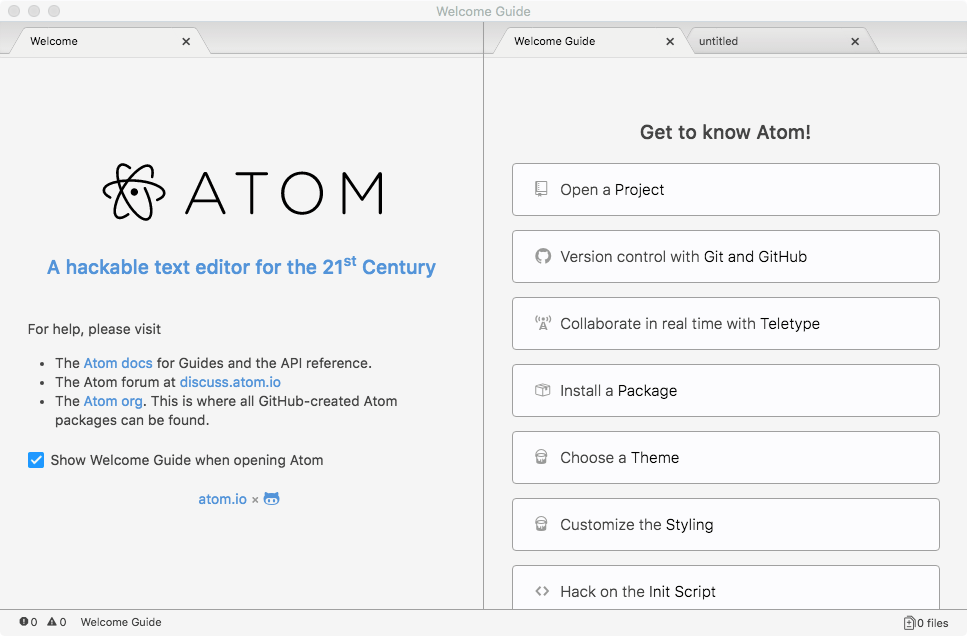
\includegraphics[scale=.2]{images/p1ch1-atomwelcome.png}}
\caption{Atom with the Welcome Guide selected}
\end{figure}

We start by creating a new project. Click on the "Open a Project" tab, and then the "Open a Project" button. A file browser pops up. Go to the Desktop, create a new folder there called "pythonadventures" and then click the "Open" button. Atom now opens a \textit{Project} pane on the right hand side. 

\begin{figure}[h]
\centerline{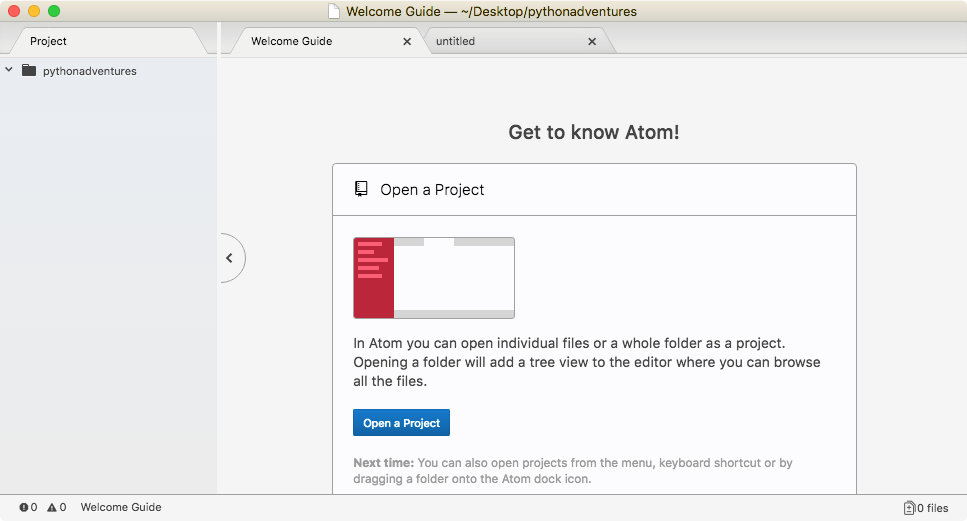
\includegraphics[scale=.20]{images/p1ch1-projectbrowser.png}}
\caption{Atom with the Project pane and browser}
\end{figure}

Next, we want to add a \texttt{git} "archive" or \emph{repository} to our project. There are two ways in which we can do that. One, we can scroll down in the Welcome Guide tab, till you see the "Version control with Git and GitHub" tab. There are two buttons there, "Open the Git panel" and "Open the GitHub panel." If you want you can click on the "Open the Git panel" -- or wait and see how we can get to that panel more quickly. If you hover with your mouse on the middle of the right side of the window, a half moon button pops up with a "$<$" inside. Click on that button to directly get to the Git panel! 

Now, because we already set up our project, the Git panel has a button that suggests we create a repository directly in our project directory. As that is exactly what we want, press the button, and then click "+Init" in the window that pops up to initialize the repository ("repo") in the directory as shown.  

Finally, select the "untitled" tab, so that we can get coding! Atom now looks like below, (and you may have noticed already that the Project browser has been updated with a ".git" folder -- our repository). 

\begin{figure}[h]
\centerline{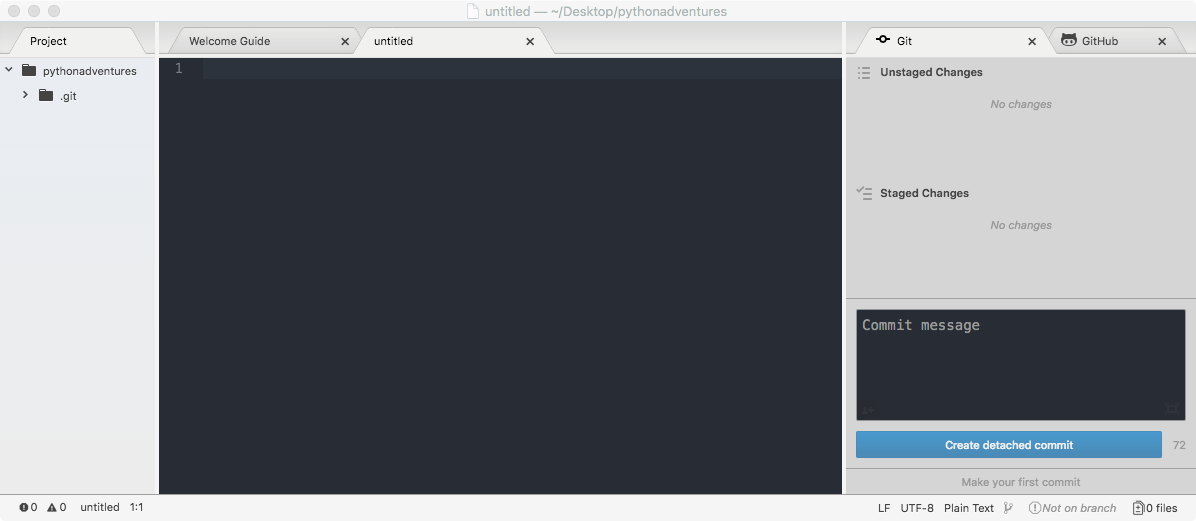
\includegraphics[scale=.20]{images/p1ch1-gituntitledprojectbrowser.png}}
\caption{Atom with the Project pane, the Git pane, and the code editor}
\end{figure} 

Type in the following lines of code in the editor. The line numbers below reflect those you see in the editor. 

\pagebreak

\begin{lstlisting}
print("You are in a dark, spooky house, all alone out in the forest.")
print("There is only one door to the outside, and it is locked.")
print("You hear strange, creaky sounds.")
\end{lstlisting}

Once you have entered the code, and save it in the project directory as \emph{p1ch1-pythonadventure.py}. In the Project panel the file now appears, and \texttt{git} has also spotted that there is something now! Notice that our file is listed under "Unstaged changes." Before \texttt{git} puts something into the repository, you need to "stage" it. Click on "Stage all" to move your file to the "stage." Then, in the \emph{Commit message} you should type a simple and short description of what is new or different in the file(s) you have staged. Right now this is simple: "everything is new!" Next, push the \emph{Commit} button. Because our repository is empty, the button says "Commit detached." Push the button, to make your first commit to the repository. Well done!

\begin{Exp}[The \texttt{git} master, and branches] 
The Commit button now says "Commit to master." The \emph{master} is the main archive. People often visualize the archive as a tree, where the main archive is the "trunk," from which you can also create "branches." A branch initially diverges from the trunk, allowing you to try things out without these experiments ending up in the main archive. This can be handy: If we decide the experiments are no good, we cut the branch and no harm is done to the main archive. If instead we decide that all is great, then we can merge the branch with the trunk to have the main archive reflect all the changes we made.      \expend 
\end{Exp}
 
\section{Letting the Player Do Something}

So the player finds himself (of herself) in a dark, spooky house. Now what ? How can we let the player do something? Most games nowadays let you move around a character in the world using a mouse, a gamepad, or a keyboard. Here, we let the user type in what he wants to do, just like players in a role-playing game like \emph{Dungeons \& Dragons} would tell the Game Master what their character is doing next! 

Type in the code below, right after the lines you just typed in. 

\begin{lstlisting}[firstnumber=last]
command = input("> ")
print("Boo!")
\end{lstlisting}

When you run the code, what happens is that the game prints the description, and then shows a prompt "$>$ " 
   
   
   
   
   
   